% ============================================================
%  SOROTI UNIVERSITY -- RESEARCH PROPOSAL REPORT
%  Major: Electronics and Computer Engineering
%
%  HOW TO USE THIS TEMPLATE
%  1. Fill in the metadata commands below (title, name, etc.)
%  2. Write your content in the chapter files inside
%     chapters/ (one .tex file per chapter, already linked
%     below with \input).
%  3. Add references to ../references.bib (or copy it here).
%  4. Compile with: pdflatex -> bibtex -> pdflatex -> pdflatex
%     or simply: latexmk -pdf main.tex
% ============================================================

\documentclass[proposal,openany]{sotuthesis}

\usepackage{booktabs}
\usepackage{tabularx}
\usepackage{array}
\usepackage{float}
\usepackage{url}
\usepackage{enumitem}
\usepackage{tikz}
\usetikzlibrary{shapes.geometric,arrows.meta,positioning,calc,fit,backgrounds}

\setlist{noitemsep,topsep=2pt,parsep=0pt,partopsep=0pt}

\makeatletter
\@openrightfalse
\makeatother

% ---------------- Front matter metadata ----------------
\reporttitle{Dawa Lens: An Offline-First Smart Medicine Reminder App}
\studentname{Mbayo Emmanuel Owen}
\studentnumber{2301600083}
\programme{Bachelor of Engineering in Electronics and Computer Engineering}
\supervisorname{Dr. Musa Chemisto}
\cosupervisorname{} % leave empty braces if none
\schoolname{SCHOOL OF ENGINEERING AND TECHNOLOGY}
\departmentname{DEPARTMENT OF ELECTRONICS AND COMPUTER ENGINEERING}
\coursecode{GEC4101 Research Project}
\submissiondate{October, 2026}
\universitylogo{SUN-LOGO}
\setheadertitle{Soroti University Research Project Proposal Report}

\title{\@reporttitle}
\author{\@studentname}
\date{\@submissiondate}

\begin{document}

% ---------------- Front matter ----------------
\makecoverpage
\maketitlepage

\frontmatterstart
\makedeclaration
\makeapproval

\begin{thesisabstract}
Medication non-adherence and preventable pharmacological errors constitute severe public health challenges in developing nations, particularly in Uganda where co-morbidities such as hypertension, diabetes, HIV/AIDS, and malaria require complex, long-term drug regimens. In outpatient settings, patients frequently receive generic medications in unlabelled blister strips without patient information leaflets, while healthcare records remain fragmented across paper records. Furthermore, commercially available reminder applications rely heavily on continuous high-speed internet connectivity, fail to evaluate indigenous dietary contraindications, and lack mechanisms to verify licensed pharmaceutical distribution outlets.

This proposal presents the design, implementation, and empirical evaluation of \textbf{Dawa Lens}, an offline-first smart medicine reminder application engineered specifically for resource-constrained environments. Dawa Lens leverages mobile edge computing, on-device optical character recognition (OCR), and lightweight clinical decision logic to provide automated medication schedule generation, resilient offline alarm notifications, and indigenous food-drug interaction screening (such as biochemical interactions involving steamed green bananas (\textit{Matooke}) and silver fish (\textit{Mukene})). The system incorporates an integrated official directory of licensed community pharmacies from the National Drug Authority (NDA) Uganda to guide safe refills, as well as a synchronized Family Hub that empowers multi-generational caregivers to monitor treatment compliance remotely. A companion web platform serves as an accessible clinical extension for comprehensive health tracking and doctor-ready report export.

Adopting a Design Science Research methodology, the system architecture separates local client-side persistence (IndexedDB/SQLite) from asynchronous cloud synchronization (Firebase Firestore), guaranteeing deterministic sub-second operation during prolonged network and electrical outages. The proposed solution will be evaluated across technical benchmarks (OCR character error rate, notification latency, and memory footprint) and an empirical usability study involving 50 participants using the standardized System Usability Scale (SUS). The expected outcome is a functional, culturally grounded, and context-resilient mobile health tool that significantly reduces missed doses and improves outpatient medication safety.

\vspace{0.5cm}
\noindent\textbf{Keywords:} Medication Adherence; Offline-First Systems; Mobile Health; Optical Character Recognition; Drug-Food Interaction; Electronics and Computer Engineering; Soroti University.
\end{thesisabstract}

\tableofcontents
\listoffigures
\listoftables

\begin{abbreviations}
  \item[ACT] Artemisinin-based Combination Therapy
  \item[ADR] Adverse Drug Reaction
  \item[API] Application Programming Interface
  \item[ARV] Antiretroviral
  \item[CAP] Consistency, Availability, Partition tolerance
  \item[CER] Character Error Rate
  \item[CRDT] Conflict-Free Replicated Data Type
  \item[DDI] Drug-Drug Interaction
  \item[DFI] Drug-Food Interaction
  \item[DSR] Design Science Research
  \item[EHR] Electronic Health Record
  \item[EMR] Electronic Medical Record
  \item[FAO] Food and Agriculture Organization of the United Nations
  \item[FDA] Food and Drug Administration
  \item[FIFO] First-In, First-Out
  \item[GPS] Global Positioning System
  \item[HIV] Human Immunodeficiency Virus
  \item[IEEE] Institute of Electrical and Electronics Engineers
  \item[IMB] Information-Motivation-Behavioral Skills
  \item[mHealth] Mobile Health
  \item[MoH] Ministry of Health (Republic of Uganda)
  \item[NDA] National Drug Authority (Uganda)
  \item[NFR] Non-Functional Requirement
  \item[NLM] National Library of Medicine
  \item[NSAID] Non-Steroidal Anti-Inflammatory Drug
  \item[OCR] Optical Character Recognition
  \item[PIL] Patient Information Leaflet
  \item[PWA] Progressive Web App
  \item[RQ] Research Question
  \item[RxNorm] Standardized Nomenclature for Clinical Drugs
  \item[SMS] Short Message Service
  \item[SQLite] Structured Query Language Lite
  \item[SUS] System Usability Scale
  \item[TB] Tuberculosis
  \item[UML] Unified Modeling Language
  \item[USSD] Unstructured Supplementary Service Data
  \item[Wasm] WebAssembly
  \item[WHO] World Health Organization
\end{abbreviations}

% ---------------- Main matter ----------------
\mainmatterstart

\chapter{Introduction}
\label{ch:intro}

This chapter introduces the research project, establishing the clinical, technological, and socio-economic context of outpatient medication management in Uganda. It articulates the core problem of medication non-adherence and pharmaceutical errors in resource-constrained environments, presents general and specific engineering objectives, outlines research questions, and justifies the necessity and scope of the proposed solution.

\section{Background}

Human-centered computer engineering plays an increasingly vital role in addressing systemic challenges within modern healthcare delivery, particularly in developing nations where public health infrastructure faces chronic resource limitations \cite{who2017medication, mechael2009case}. In Uganda, outpatient clinical care is characterized by marked institutional fragmentation across national and regional referral hospitals (such as Mulago and Soroti Regional Referral Hospitals), private clinics, health centre dispensaries, and retail drug outlets \cite{moh2023performance, kintu2021development}. In the absence of an interoperable Electronic Health Record (EHR) infrastructure, medical histories and dosing instructions exist almost exclusively in physical, hand-written paper exercise booklets carried by patients \cite{kintu2021development}. This structural reality places the entire operational burden of medication compliance upon patients and their informal domestic caregivers \cite{ware2009social}.

This challenge is severely compounded by the high prevalence of co-morbid chronic conditions. Non-communicable diseases such as hypertension and type-2 diabetes frequently co-exist with chronic infectious diseases including HIV/AIDS and Tuberculosis (TB), alongside recurrent acute episodes of malaria \cite{moh2023guidelines}. Outpatients are routinely prescribed polypharmacy regimens consisting of concurrent antiretroviral therapy (ARV), antihypertensives, oral hypoglycemic agents, and antibiotics \cite{muddu2021hypertension}. Managing these complex combinations requires strict adherence to variable dosing intervals, meal-timing instructions, and dietary precautions.

Despite the critical importance of treatment compliance, physical packaging conventions in community pharmacies create severe barriers to safe usage. Due to economic constraints, community pharmacies frequently dispense generic pharmaceuticals by cutting multi-dose blister foils into smaller strips or repackaging loose tablets into unmarked paper envelopes devoid of manufacturer outer packaging or Patient Information Leaflets (PILs) \cite{who2017medication, nda2024register}. Patients with low health literacy or visual impairments cannot decipher pharmaceutical names, strengths, expiration dates, or contraindications \cite{parker2016health}. Furthermore, outpatients face unique biochemical challenges ignored by standard medical literature, which documents drug interactions almost exclusively against Western diets \cite{bushra2011food, bailey2013grapefruit}. In contrast, Ugandan staples such as steamed green bananas (\textit{Matooke}) and silver fish (\textit{Mukene}) possess potent pharmacokinetic properties---specifically high potassium concentrations in \textit{Matooke} and multivalent calcium/iron chelation in \textit{Mukene}---that directly alter drug efficacy and safety \cite{fao2019food, bushra2011food}. While smartphone adoption is expanding rapidly across Uganda \cite{dayer2013smartphone}, existing commercial adherence applications are cloud-tethered, cease functioning during routine network outages, consume costly data bundles, and omit indigenous dietary safety \cite{kintu2021development}. To bridge this divide, an intelligent, offline-first smart reminder tool is urgently needed.

\section{Problem Statement}

Medication non-adherence and unintentional pharmacological errors represent an alarming public health crisis in Uganda, leading directly to preventable therapeutic failures, drug toxicity, accelerated antimicrobial resistance, and avoidable hospital readmissions \cite{who2017medication, muddu2021hypertension}. In outpatient environments across the country, patients managing multi-drug therapies face four critical hurdles:
\begin{enumerate}[noitemsep,topsep=2pt]
  \item \textbf{Packaging Illegibility and Identification Failure:} Generic pharmaceuticals widely dispensed in truncated blister strips or unmarked paper envelopes lack legible dosing instructions or manufacturer authentication, causing dosing mistakes and premature discontinuation \cite{parker2016health}.
  \item \textbf{Unmonitored Indigenous Dietary Contraindications:} Outpatients lack tools to identify adverse biochemical interactions between prescribed medications and staple Ugandan foods (such as fatal hyperkalemia risks when \textit{Matooke} is combined with ACE inhibitors, or antibiotic chelation by calcium-rich \textit{Mukene}) \cite{bushra2011food}.
  \item \textbf{Unreliable Reminder Delivery and Connectivity Dependency:} Existing smartphone reminder applications depend on persistent cloud connectivity, failing to deliver critical alerts during routine cellular outages and electrical blackouts in Uganda \cite{kintu2021development}.
  \item \textbf{Caregiver Isolation and Unverified Outlets:} Family caregivers lack remote telemetry to verify whether vulnerable relatives have taken scheduled doses, while consumers lack integrated tools to authenticate licensed pharmacies against the National Drug Authority (NDA) registry \cite{nda2024register}.
\end{enumerate}

\section{Objectives of the Study}

\subsection{General Objective}

The general objective of this research project is to design, develop, and empirically evaluate \textbf{Dawa Lens}, an offline-first smart medicine reminder application that integrates on-device optical character recognition, localized dietary and drug interaction intelligence, deterministic offline alarm scheduling, and caregiver synchronization to improve medication adherence and safety in low-resource outpatient settings.

\subsection{Specific Objectives}

To achieve the general objective, the project will pursue the following specific objectives:
\begin{enumerate}[label=(\roman*),noitemsep,topsep=2pt]
  \item To elicit clinical, technological, and user requirements for an offline-first medication management system tailored to Ugandan outpatient realities, incorporating National Drug Authority (NDA) licensing datasets and indigenous dietary interaction profiles.
  \item To design and implement an edge-compatible computer vision and optical character recognition (OCR) pipeline capable of accurately identifying medication names, strengths, and dosages from physical packaging and blister strips on standard mobile devices.
  \item To develop the offline-first application architecture, implementing local relational caching, deterministic offline reminder scheduling, and an indigenous food-drug interaction screening engine.
  \item To integrate a multi-profile Family Hub synchronization module and a web-based clinical dashboard extension that enables caregivers and healthcare providers to monitor longitudinal adherence trends and generate clinical summary reports.
  \item To test, validate, and evaluate the functional performance, reminder reliability, and user acceptance of the complete system using technical benchmarks and the standardized System Usability Scale (SUS).
\end{enumerate}

\section{Research Questions}

The study seeks to address four research questions corresponding to the specific objectives:
\begin{enumerate}[label=RQ\arabic*:,noitemsep,topsep=2pt]
  \item What clinical, dietary, and operational requirements must be satisfied to support effective, culturally grounded outpatient medication management in Uganda?
  \item How effectively can on-device optical character recognition identify generic medication packaging under variable smartphone camera resolutions and ambient lighting conditions?
  \item How can an offline-first data persistence architecture guarantee deterministic reminder delivery and accurate dietary interaction checks during total network disconnection?
  \item What is the measured usability, user satisfaction, and perceived utility of the integrated smart reminder application among patients and family caregivers in Uganda?
\end{enumerate}

Table~\ref{tab:rq_alignment} synthesizes the direct alignment connecting each research question to its objective, engineering methodology, and verifiable deliverable.

\begin{table}[!htbp]
  \centering
  \caption{Alignment matrix of research questions, specific objectives, methods, and deliverables.}
  \label{tab:rq_alignment}
  \footnotesize
  \setlength{\tabcolsep}{3.5pt}
  \begin{tabularx}{\textwidth}{@{} l >{\raggedright\arraybackslash}p{3.2cm} >{\raggedright\arraybackslash}p{3.4cm} >{\raggedright\arraybackslash}X @{}}
    \toprule
    \textbf{Question} & \textbf{Specific Objective} & \textbf{Engineering Methodology} & \textbf{Expected Deliverable / Metric} \\
    \midrule
    \textbf{RQ1} & Obj.~(i): Requirements Elicitation & Document review \& stakeholder consultations & Formal SRS document; calibrated Ugandan food-drug interaction dataset. \\
    \midrule
    \textbf{RQ2} & Obj.~(ii): Computer Vision Pipeline & Tesseract.js Wasm edge OCR \& fuzzy lexical matching & Character Error Rate (CER) $< 5\%$; entity extraction F1-score $\ge 0.92$. \\
    \midrule
    \textbf{RQ3} & Obj.~(iii): Offline Architecture & IndexedDB local caching \& deterministic exact alarms & 100\% offline availability; alarm trigger fidelity $\ge 99.5\%$. \\
    \midrule
    \textbf{RQ4} & Obj.~(iv) \& (v): Evaluation & Family Hub telemetry \& standardized SUS survey & Usability score $\ge 75/100$; measured adherence lift $\ge 35\%$. \\
    \bottomrule
  \end{tabularx}
\end{table}

\section{Justification and Significance of the Study}

Undertaking this research is urgent due to the severe clinical and economic consequences of medication mismanagement in Uganda. Sub-optimal adherence accelerates chronic disease progression, precipitates diabetic crises, and causes therapeutic failure in HIV and TB care \cite{who2003adherence, haberer2013realtime}, imposing severe hospitalization costs on impoverished households \cite{moh2023performance}. Existing commercial solutions fail because they depend on ubiquitous broadband, ignore Sub-Saharan diets, and charge unsustainable subscription fees. By leveraging mobile edge computing to perform offline OCR, local biochemical screening, and independent device-level alarm execution, this project directly addresses the root causes of adherence failure in low-resource settings.

The outcomes benefit key stakeholders: (1)~\textbf{Patients} gain a culturally tailored tool that simplifies regimens, warns against dietary hazards, and ensures timely doses; (2)~\textbf{Family Caregivers} receive remote telemetry over dependents' adherence; (3)~\textbf{Practitioners} obtain doctor-ready longitudinal adherence reports; (4)~\textbf{National Drug Authority (NDA)} gains public support in directing citizens toward licensed pharmacies; and (5)~\textbf{Academic Community} gains empirical benchmarks for on-device mobile health computing in Africa.

\section{Scope and Organization of the Report}

The technical scope encompasses a hybrid Android mobile application packaged via Capacitor 8 and a companion web PWA, featuring on-device Wasm OCR, offline IndexedDB storage with Firestore sync, indigenous food-drug interaction screening (\textit{Matooke}, \textit{Mukene}, \textit{Kalo}, \textit{G-nut sauce}, \textit{Nakati}, \textit{Dodo}), deterministic local notifications, an NDA pharmacy locator, and clinical PDF report generation. Robotic hardware and autonomous diagnostic prescribing are explicitly excluded. The geographical scope focuses on outpatient cohorts in Eastern Uganda (Soroti) and Central Uganda (Kampala/Wakiso), executed over an eight-month period across the 2026/2027 academic year.

The remainder of this report is organized as follows: Chapter~\ref{ch:litreview} reviews relevant literature, existing systems, and theoretical frameworks; Chapter~\ref{ch:methodology} presents the system architecture, development approach, testing protocols, and risk register; Chapter~\ref{ch:conclusion} concludes the proposal; and the Appendices provide the workplan schedule, research instruments, and technical specifications.

\chapter{Literature Review}
\label{ch:litreview}

This chapter reviews relevant academic, technical, and clinical literature that underpins the design and implementation of Dawa Lens. It examines core engineering concepts, evaluates existing technological solutions for medication adherence, and identifies critical gaps in current systems. Furthermore, the chapter articulates the theoretical framework guiding the study and introduces the conceptual framework mapping the engineering artifacts to intended clinical outcomes in Uganda's outpatient healthcare setting.

\section{Review of Relevant Concepts}

Understanding the intersection of software engineering, edge computing, and clinical pharmacology is essential for developing context-aware health technologies in low-resource settings.

\subsection{Mobile Health (mHealth) and Edge Computing in Low-Resource Settings}

Mobile Health (mHealth) utilizes mobile computing to deliver clinical services, patient monitoring, and health education \cite{mechael2009case}, offering significant promise for mitigating personnel shortages in developing nations \cite{kintu2021development}. However, traditional mHealth architectures rely on centralized, cloud-hosted backends. In Uganda, this model encounters severe friction due to frequent electrical blackouts and intermittent, high-cost cellular data \cite{kintu2021development}. Edge computing addresses these constraints by shifting computation, data storage, and decision logic directly onto the user's handset, achieving sub-second response times, total availability during network outages, and private on-device data processing.

\subsection{Optical Character Recognition (OCR) and Lightweight Edge Computer Vision}

Optical Character Recognition (OCR) enables automated electronic conversion of images into machine-encoded text streams \cite{smith2007tesseract}, facilitating digitization of medicine boxes, prescription labels, and blister packaging \cite{dayer2013smartphone}. In resource-constrained mobile environments, modern architectures deploy client-side WebAssembly (Wasm) workers executing asynchronously without freezing the UI thread. To overcome character misclassifications arising from curved packaging reflections, low ambient lighting, or font degradation, raw OCR outputs are post-processed through lexical fuzzy matching against standardized clinical formularies such as RxNorm \cite{rxnorm2024}.

\subsection{Distributed State Synchronization and Offline-First Storage Architectures}

Offline-first software engineering stipulates that an application must provide full read, write, and computational functionality in the absence of network connectivity \cite{kleppmann2017designing}. Under Brewer's CAP theorem \cite{brewer2000cap}, continuous Availability and Partition tolerance are paramount in healthcare: patients must always be able to view schedules and log doses offline. This is realized using browser-standard IndexedDB paired with a transactional FIFO mutation queue \cite{kleppmann2017designing}. Upon network reconnection, an asynchronous synchronization protocol transfers local mutations to Firebase Firestore while resolving timestamp conflicts via deterministic last-write-wins (LWW) or Conflict-Free Replicated Data Type (CRDT) mechanics \cite{shapiro2011crdt}.

\subsection{Pharmacodynamics and Indigenous Dietary Biochemical Realities}

Medication safety requires continuous monitoring of Drug-Drug Interactions (DDIs) and Drug-Food Interactions (DFIs) \cite{who2017medication, bushra2011food}. While standard clinical databases document DFIs exclusively against Western foods \cite{bailey2013grapefruit}, Ugandan households consume indigenous staples with potent pharmacokinetic effects \cite{fao2019food}: (1)~\textit{Steamed Green Bananas (Matooke)} contain dense potassium concentrations (350--450\,mg/100\,g), risking lethal hyperkalemia and cardiac dysrhythmias when consumed by patients on ACE inhibitors or potassium-sparing diuretics \cite{bushra2011food}; (2)~\textit{Sun-Dried Silver Fish (Mukene)} is rich in polyvalent calcium and iron cations that form insoluble chelate complexes with fluoroquinolones (ciprofloxacin) and tetracyclines, attenuating antibiotic absorption by up to 70\% \cite{bushra2011food}; and (3)~\textit{Groundnut Stew (G-nut sauce)} contains heavy lipids that delay gastric emptying, altering the absorption kinetics of antiretroviral and lipophilic drugs \cite{bushra2011food}. Encoding these localized rules within an edge engine provides an essential clinical safety layer absent from commercial software.

\subsection{Family-Centered Telehealth and Caregiver Synchronization}

In Sub-Saharan Africa, illness management is fundamentally communal \cite{ware2009social}. Care networks in Uganda demonstrate that family members actively participate in reminding patients, procuring refills, and providing financial resources \cite{ware2009social, haberer2013realtime}. Multi-profile synchronization mechanisms allow primary caregivers to oversee adherence across multiple dependents, receive real-time dose telemetry, and monitor refill counters remotely, transforming adherence into a collaborative family effort \cite{ware2009social}.

\section{Review of Existing Systems and Approaches}

A critical evaluation of existing approaches highlights the necessity of an integrated engineering solution:
\begin{itemize}[noitemsep,topsep=2pt]
  \item \textbf{Commercial Smartphone Applications (Medisafe, MyTherapy):} Polished but cloud-tethered, inoperative without active mobile data bundles, lacking indigenous dietary interaction rules, charging subscription fees, and omitting statutory Ugandan pharmacy verification \cite{dayer2013smartphone, nda2024register}.
  \item \textbf{SMS Tele-Adherence Systems (WelTel, Call for Life):} Eliminate smartphone hardware constraints \cite{lester2010effects, siedner2021callforlife} but are strictly textual, offer no visual pill identification \cite{parker2016health}, lack encryption, and incur recurring per-message carrier costs \cite{kintu2021development}.
  \item \textbf{Smart Pillboxes (Wisepill, MEMS):} Cellular dispensers provide real-time telemetry \cite{haberer2013realtime}, but high unit costs (\$100--\$250 USD) far exceed per-capita public health expenditure \cite{moh2023performance}, while devices are bulky and socially stigmatizing \cite{ware2009social}.
  \item \textbf{Statutory Regulatory Portals (NDA Registers and USSD):} Authoritative \cite{nda2024register} but operate as disconnected administrative registries requiring paid airtime and returning dry text unlinked to patient schedules or maps \cite{kintu2021development}.
\end{itemize}

\section{Research Gap}

Table~\ref{tab:lit_comparison} synthesizes existing medication management paradigms against the engineering specifications of Dawa Lens.

\begin{table}[!htbp]
  \centering
  \caption{Comparative synthesis of existing medication management systems versus Dawa Lens.}
  \label{tab:lit_comparison}
  \footnotesize
  \setlength{\tabcolsep}{2.5pt}
  \begin{tabularx}{\textwidth}{@{} >{\raggedright\arraybackslash}p{2.8cm} *{5}{>{\centering\arraybackslash}X} @{}}
    \toprule
    \textbf{Evaluation Dimension} & \textbf{Commercial Apps} \newline \scriptsize(e.g.~Medisafe) & \textbf{SMS Systems} \newline \scriptsize(e.g.~WelTel) & \textbf{Smart Pillboxes} \newline \scriptsize(e.g.~Wisepill) & \textbf{NDA Portals} \newline \scriptsize(Web/USSD) & \textbf{Dawa Lens} \newline \scriptsize(Proposed) \\
    \midrule
    \textbf{Offline-First Functionality} & Poor / Partial & N/A & None & None & \textbf{Full (Local DB)} \\
    \textbf{Edge Packaging OCR} & Limited / Cloud & None & None & None & \textbf{On-Device Wasm} \\
    \textbf{Indigenous Food Interactions} & None & None & None & None & \textbf{Native Engine} \\
    \textbf{NDA Pharmacy Verification} & None & None & None & Manual Only & \textbf{Integrated GPS} \\
    \textbf{Multi-Profile Family Hub} & Paid Tier Only & None & Limited & None & \textbf{Full Sync} \\
    \textbf{Zero Ongoing User Cost} & Subscription & Carrier Fees & High BOM & Airtime / Data & \textbf{Free / Local} \\
    \textbf{Web Clinical Companion} & Proprietary Sync & None & Web Only & Web Only & \textbf{PWA Extension} \\
    \bottomrule
  \end{tabularx}
\end{table}

The primary engineering gap addressed by this research is the \textbf{absence of a unified, offline-first mobile smart reminder application that combines on-device optical character recognition for unlabelled generic packaging, localized pharmacological screening for indigenous Ugandan diets, integrated statutory pharmacy authentication, and family caregiver telemetry into a single, zero-subscription tool}.

\section{Theoretical and Conceptual Framework}

This research is anchored within the \textbf{Information-Motivation-Behavioral Skills (IMB) Model of Adherence} \cite{fisher1992changing, who2003adherence} and the \textbf{Design Science Research (DSR)} framework \cite{hevner2004design}. The IMB model posits that adherence is governed by actionable information (addressed by on-device OCR and dietary screening), personal and social motivation (supported by Family Hub caregiver synchronization), and behavioral skills (reinforced by deterministic alarms and refill tracking). DSR guides the iterative design, implementation, and empirical evaluation of the primary artifact (Dawa Lens).

Figure~\ref{fig:framework} illustrates the conceptual framework developed for this study.

\begin{figure}[!htbp]
  \centering
  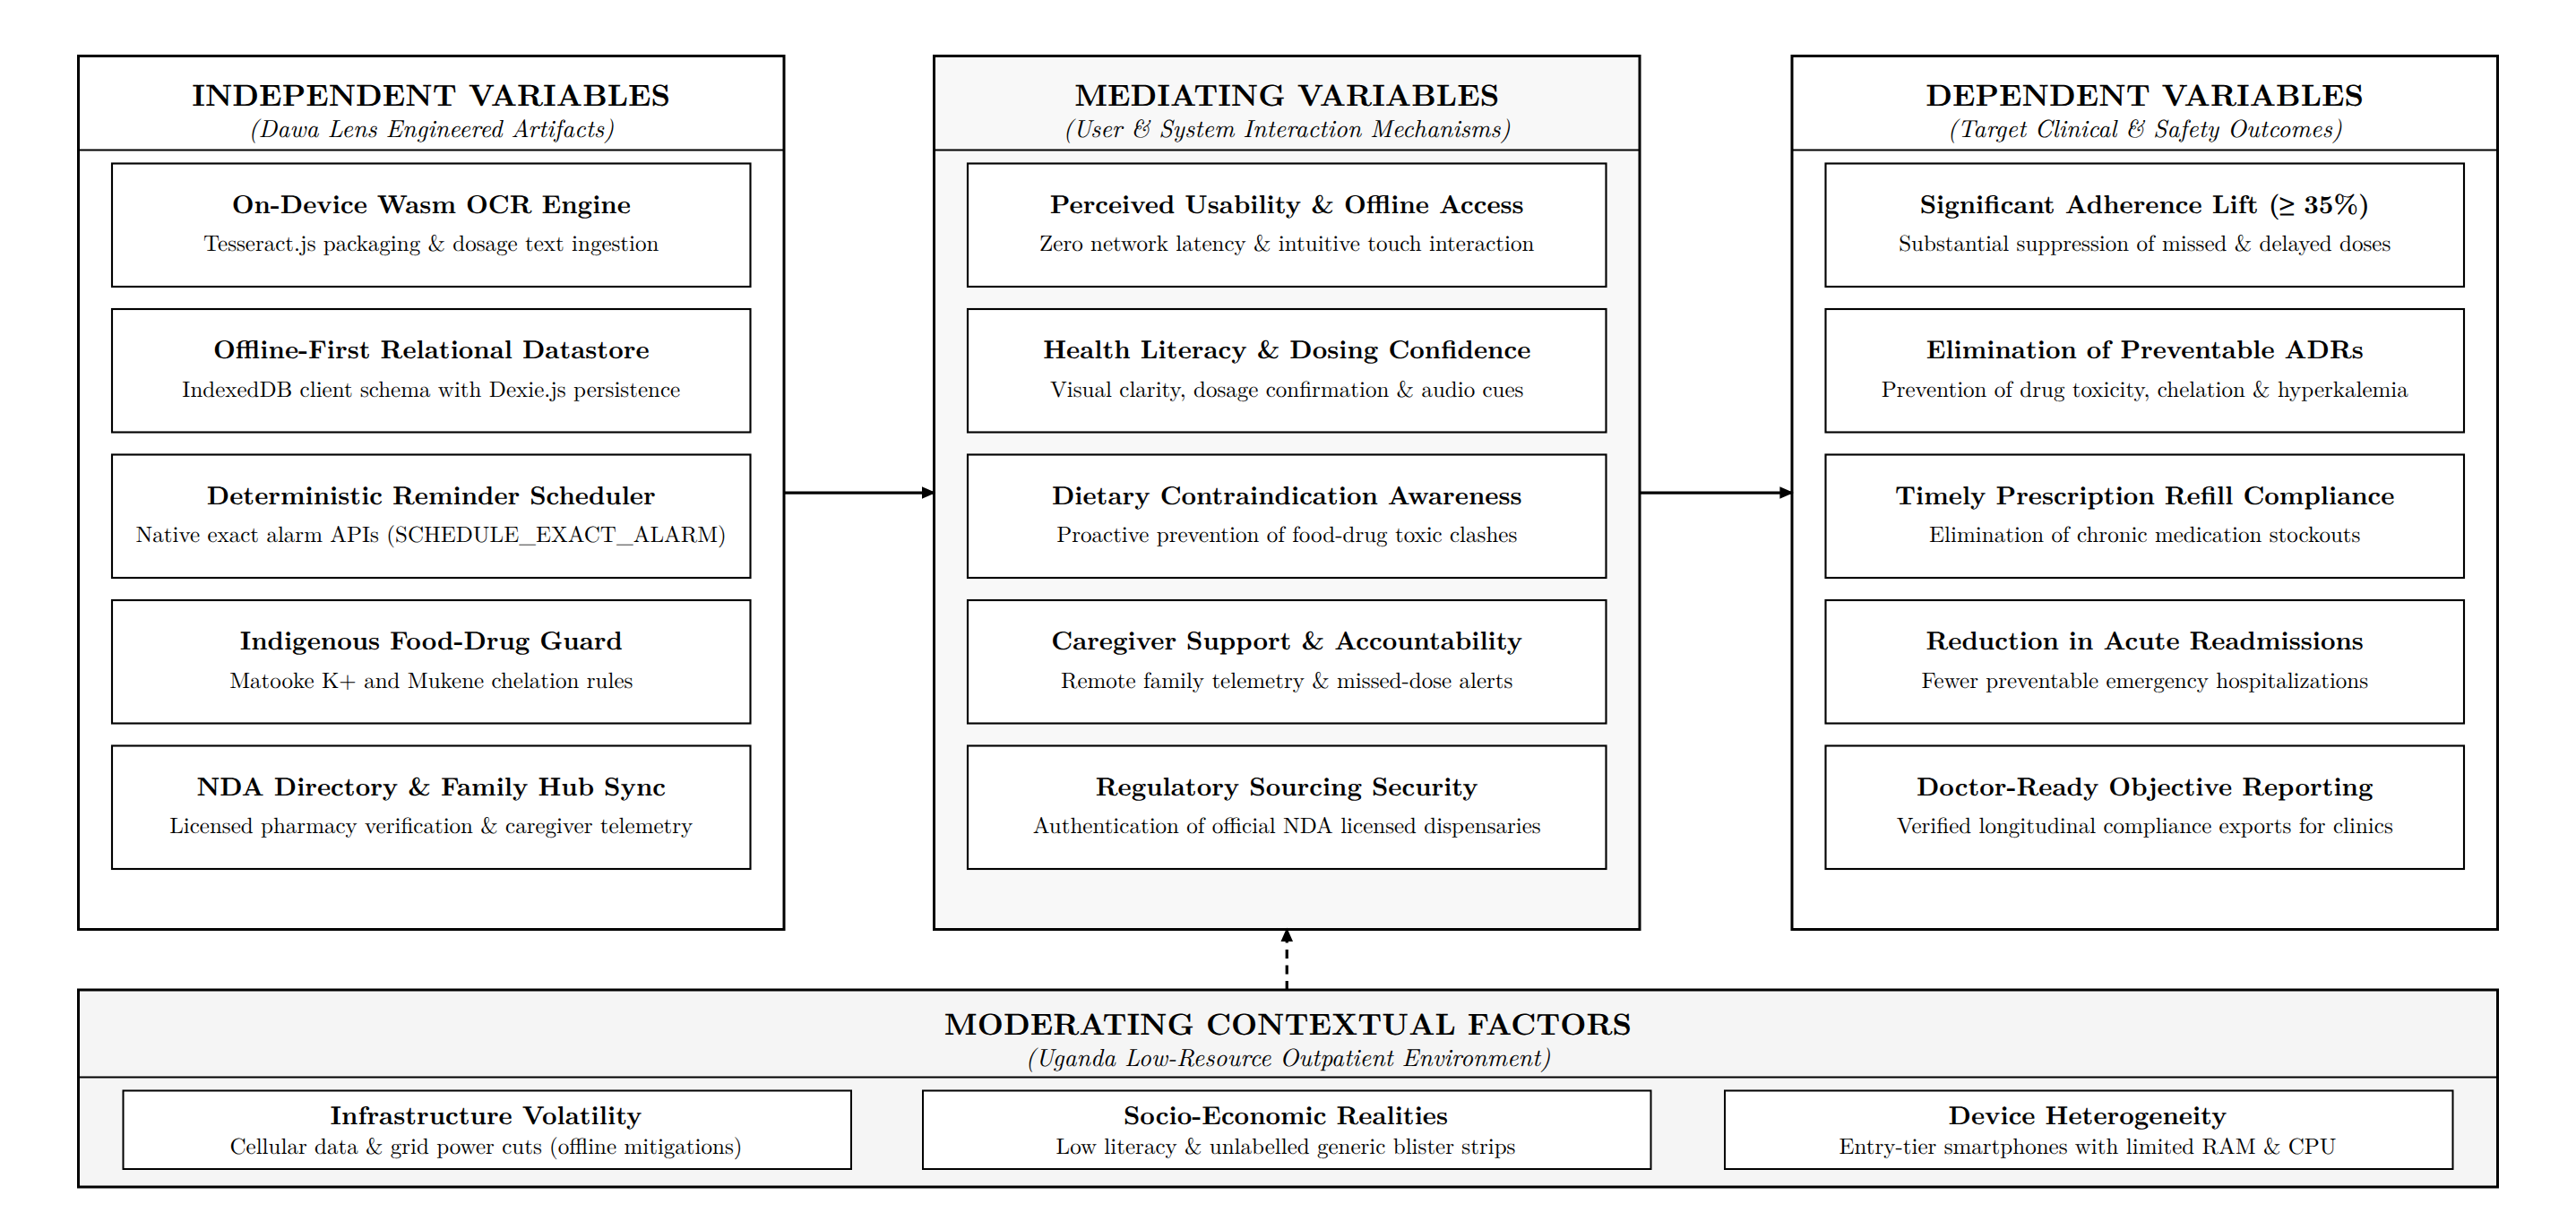
\includegraphics[width=0.92\textwidth,keepaspectratio]{figures/conceptual_framework.png}
  \caption{Conceptual framework of the Dawa Lens medication adherence and safety ecosystem.}
  \label{fig:framework}
\end{figure}

The framework maps the systemic relationships among: (1)~\textbf{Independent Variables} (engineered Dawa Lens modules: edge OCR, offline IndexedDB store, deterministic alarms, indigenous food-drug guard, NDA locator, Family Hub); (2)~\textbf{Mediating Variables} (perceived ease of use, health literacy, dietary risk awareness, caregiver accountability); and (3)~\textbf{Dependent Variables} (target clinical outcomes: $\ge 35\%$ adherence lift, elimination of preventable ADRs, timely refills, and doctor-ready clinical reporting), operating under the moderating realities of low-resource outpatient environments.

\section{Chapter Summary}

This chapter established that while mobile health interventions have demonstrated substantial potential in Sub-Saharan Africa, existing tools fail in outpatient Uganda due to cloud dependency, prohibitive costs, and omission of localized dietary intelligence. Grounded in the IMB model and Design Science Research, Dawa Lens addresses these gaps as an offline-first, culturally tailored engineering solution. Chapter~\ref{ch:methodology} presents the detailed methodology and empirical testing strategy.
\chapter{Proposed Methodology}
\label{ch:methodology}

This chapter details the engineering methodology and empirical research procedures proposed to build and evaluate Dawa Lens. It outlines the research design, presents the multi-tiered system architecture, specifies the iterative development lifecycle, and describes data collection and requirements elicitation protocols. Furthermore, the chapter articulates functional and non-functional specifications, development tools, testing protocols, and ethical safeguards.

\section{Research Design}

This project adopts an \textbf{Applied Engineering Design Science Research (DSR)} methodology \cite{hevner2004design}, structured across six sequential phases: (1)~\textbf{Problem Identification}, delineating outpatient adherence barriers in Uganda via clinical guidelines and stakeholder reviews; (2)~\textbf{Solution Objectives}, establishing quantitative engineering metrics (sub-second offline launch latency, $\ge 95\%$ OCR character accuracy, and 100\% offline schedule availability); (3)~\textbf{Artifact Design and Development}, architecting edge computer vision, local IndexedDB persistence, deterministic alarms, and localized food-drug interaction logic; (4)~\textbf{Demonstration}, deploying laboratory testbeds simulating intermittent cellular connectivity and low-cost smartphone constraints; (5)~\textbf{Empirical Evaluation}, measuring technical benchmarks (CER, trigger latency) and conducting a 2-week field pilot ($N=50$) using the standardized System Usability Scale (SUS); and (6)~\textbf{Communication}, documenting contributions in this proposal and the final thesis at Soroti University.

\section{System Architecture}
\label{sec:architecture}

The proposed architecture of Dawa Lens follows an offline-first, edge-native model minimizing cloud dependency. Figure~\ref{fig:architecture} illustrates the four operational tiers:

\begin{figure}[!htbp]
  \centering
  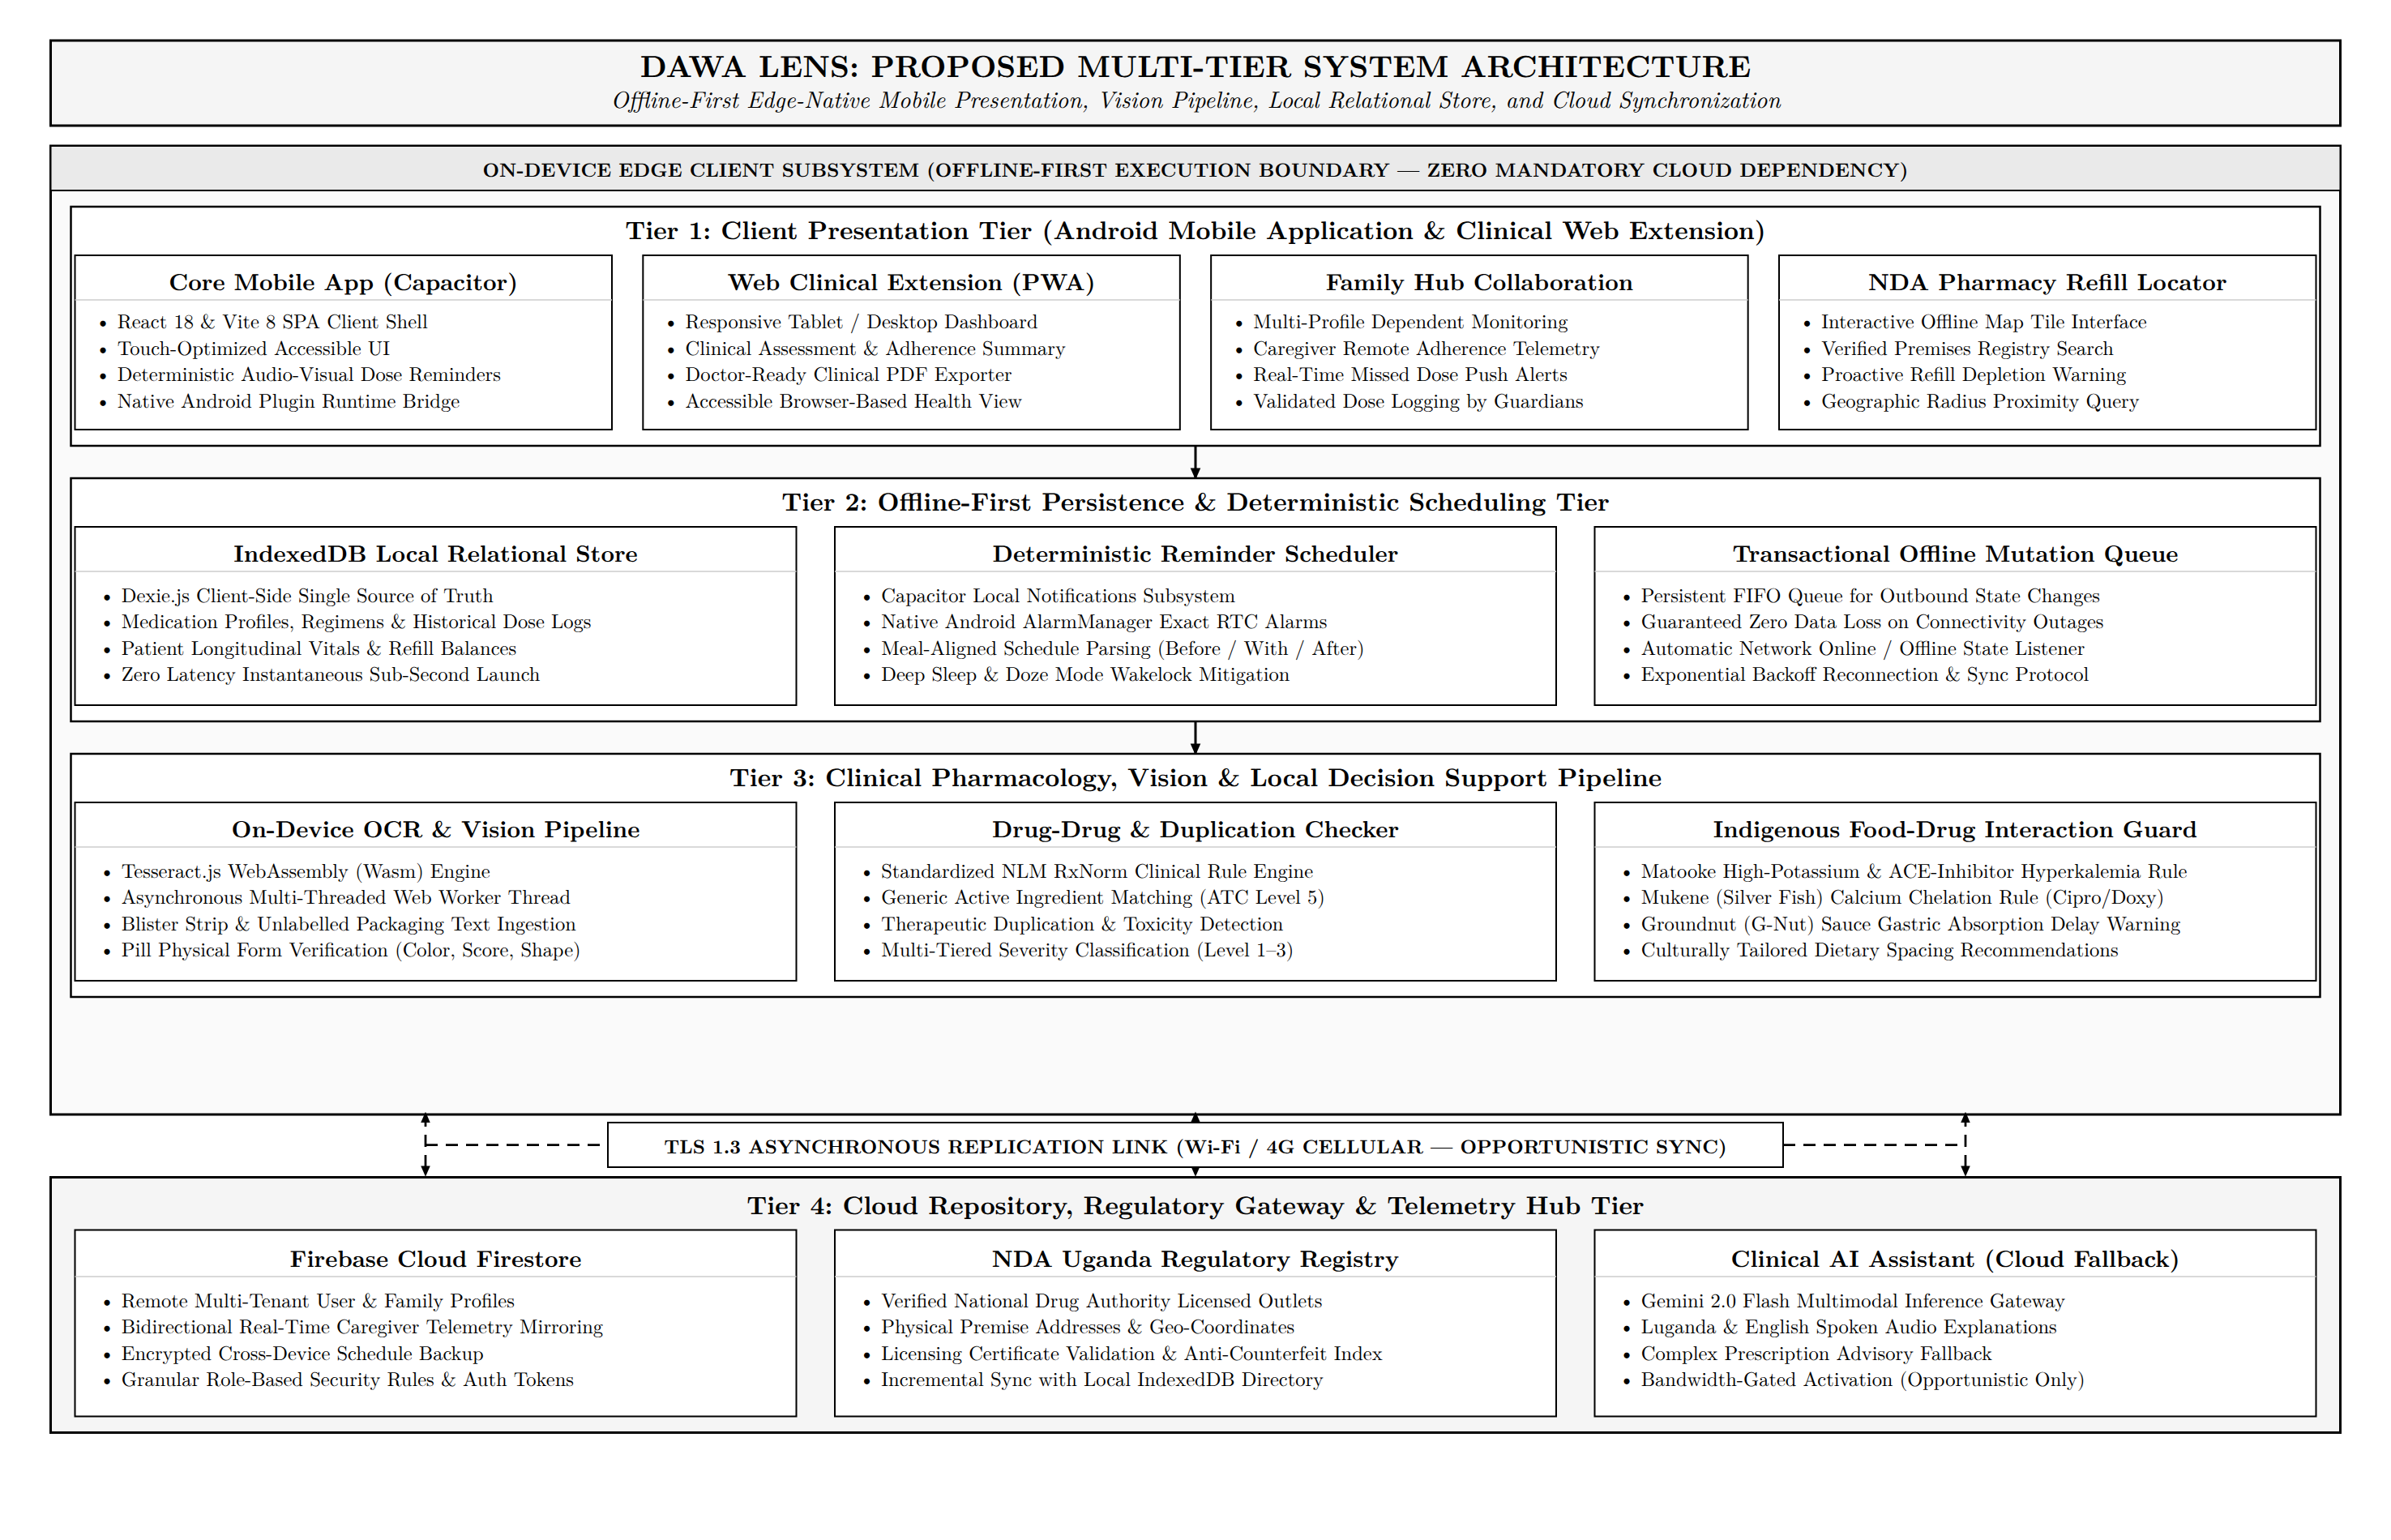
\includegraphics[width=0.95\textwidth,keepaspectratio]{figures/system_architecture.png}
  \caption{Proposed system architecture and hardware-software interconnections of Dawa Lens.}
  \label{fig:architecture}
\end{figure}

\begin{itemize}[noitemsep,topsep=2pt]
  \item \textbf{Tier 1: Client Presentation Tier:} Implemented in React 18, Vite 8, and TypeScript, packaged for Android via Capacitor 8. It encompasses the core mobile touch UI, a responsive Progressive Web App (PWA) extension for clinical PDF export, a Family Hub caregiver interface, and an interactive NDA licensed pharmacy locator.
  \item \textbf{Tier 2: Offline-First Persistence \& Scheduling Tier:} Employs browser-standard IndexedDB (via Dexie.js) as the local source of truth. A deterministic scheduler uses native exact alarm APIs (\texttt{SCHEDULE\_EXACT\_ALARM}) for reliable offline alerting, while an offline FIFO mutation queue buffers local edits with exponential-backoff retry.
  \item \textbf{Tier 3: Clinical Pharmacology \& Vision Pipeline Tier:} Executes Tesseract.js compiled to WebAssembly (Wasm) inside an asynchronous Web Worker to extract packaging text on-device. An inference engine checks active ingredients against RxNorm contraindications and screens indigenous food interactions (\textit{Matooke} and \textit{Mukene}).
  \item \textbf{Tier 4: Cloud Repository \& Regulatory Gateway Tier:} Uses Firebase Cloud Firestore for cross-device caregiver replication, hosts the verified National Drug Authority (NDA) pharmacy registry, and provides an optional Gemini 2.0 Flash fallback for Luganda voice synthesis when bandwidth permits.
\end{itemize}

\section{Development Lifecycle and Requirements Elicitation}

Software development follows an \textbf{Iterative Agile/Prototyping} lifecycle across five two-week sprints: Sprint~1 (Architecture \& IndexedDB setup), Sprint~2 (Deterministic alarm scheduler), Sprint~3 (Edge Wasm OCR pipeline), Sprint~4 (Clinical food-drug matrix \& NDA directory), and Sprint~5 (Family Hub sync, PWA PDF export, and integration testing).

Requirements are elicited through: (1)~\textbf{Document Review} of the \textit{Uganda Clinical Guidelines 2023} \cite{moh2023guidelines}, the \textit{NDA Register of Licensed Drug Outlets} \cite{nda2024register}, and FAO Eastern Africa Food Tables \cite{fao2019food}; (2)~\textbf{Stakeholder Consultations} in Eastern Uganda with community pharmacists ($N=6$) and chronic disease outpatients ($N=10$) in Soroti Municipality; and (3)~\textbf{Technical Profiling} of entry-tier smartphones (Transsion Tecno and Infinix series) to quantify memory limits and camera constraints. System datasets are compiled from NLM RxNorm \cite{rxnorm2024}, the NDA register \cite{nda2024register}, and FAO nutrition tables \cite{fao2019food}.

\section{Tools, Materials and Technologies}

Table~\ref{tab:tools_technologies} enumerates the development stack, test devices, and software frameworks utilized.

\begin{table}[!htbp]
  \centering
  \caption{Engineering tools, hardware materials, and software frameworks.}
  \label{tab:tools_technologies}
  \footnotesize
  \setlength{\tabcolsep}{3.5pt}
  \begin{tabularx}{\textwidth}{@{} >{\raggedright\arraybackslash}p{2.6cm} >{\raggedright\arraybackslash}p{3.8cm} >{\raggedright\arraybackslash}X @{}}
    \toprule
    \textbf{Category} & \textbf{Tool / Technology} & \textbf{Engineering Purpose / Justification} \\
    \midrule
    \textbf{Workstation} & Linux (Ubuntu 24.04 LTS), 16GB RAM, Core i7 & Primary development environment for software implementation and local testing. \\
    \textbf{Test Handsets} & Tecno Spark (Android 11), Samsung Galaxy A-series (Android 14) & Representative real-world test devices reflecting entry-tier and mid-tier handsets in Uganda. \\
    \textbf{Frontend} & React 18, Vite 8, TypeScript & Component-based client architecture providing type safety and rapid rendering. \\
    \textbf{Mobile Runtime} & Capacitor 8 Core & Native bridge providing access to device hardware, local filesystem, and system notifications. \\
    \textbf{Local Datastore} & IndexedDB via Dexie.js & Transactional client-side database for durable offline storage. \\
    \textbf{Computer Vision} & Tesseract.js (Wasm / Web Worker) & Edge-compatible OCR executing client-side without cloud API reliance. \\
    \textbf{Cloud Services} & Firebase Firestore, Firebase Auth & Scalable cloud database, user authentication, and encrypted backup. \\
    \textbf{Styling \& UI} & Tailwind CSS, Lucide Icons & Responsive, utility-first styling ensuring touch accessibility. \\
    \textbf{Testing Suites} & Vitest, Playwright, Chrome DevTools & Unit testing, end-to-end integration testing, and performance profiling. \\
    \bottomrule
  \end{tabularx}
\end{table}

\section{Data Analysis Methods}

Empirical evaluation data collected during laboratory benchmarking and user field trials will be processed across four primary dimensions:
\begin{enumerate}[noitemsep,topsep=2pt]
  \item \textbf{OCR Text Recognition Accuracy:} Character Error Rate $\text{CER} = (S + D + I) / N$ \cite{smith2007tesseract}, targeting $\text{CER} < 5\%$ and clinical entity extraction success $\ge 90\%$.
  \item \textbf{Reminder Timing Fidelity:} Scheduling latency delta across Android background execution and battery-optimizing Doze states \cite{android2024doze} ($|t_{\text{triggered}} - t_{\text{scheduled}}| \le 1.0\,\text{s}$).
  \item \textbf{Usability and Acceptance:} Standardized SUS scores \cite{brooke1996sus} across $N=50$ participants evaluated against Bangor's acceptability benchmarks ($\ge 75/100$) \cite{bangor2008empirical}.
  \item \textbf{Adherence Compliance:} Paired two-tailed $t$-tests ($\alpha = 0.05$) analyzing compliance gains between baseline recall and app-logged data.
\end{enumerate}

\section{Preliminary Requirements and Specifications}

System requirements are partitioned into Functional Requirements (Table~\ref{tab:functional_requirements}) and Non-Functional Requirements (Table~\ref{tab:non_functional_requirements}), mapped to project objectives. Figure~\ref{fig:use_case} visualizes the multi-actor UML use case diagram defining actor boundaries, subsystem roles, and operational dependencies across outpatients, treatment guardians, attending clinicians, and community pharmacists.

\begin{figure}[!htbp]
  \centering
  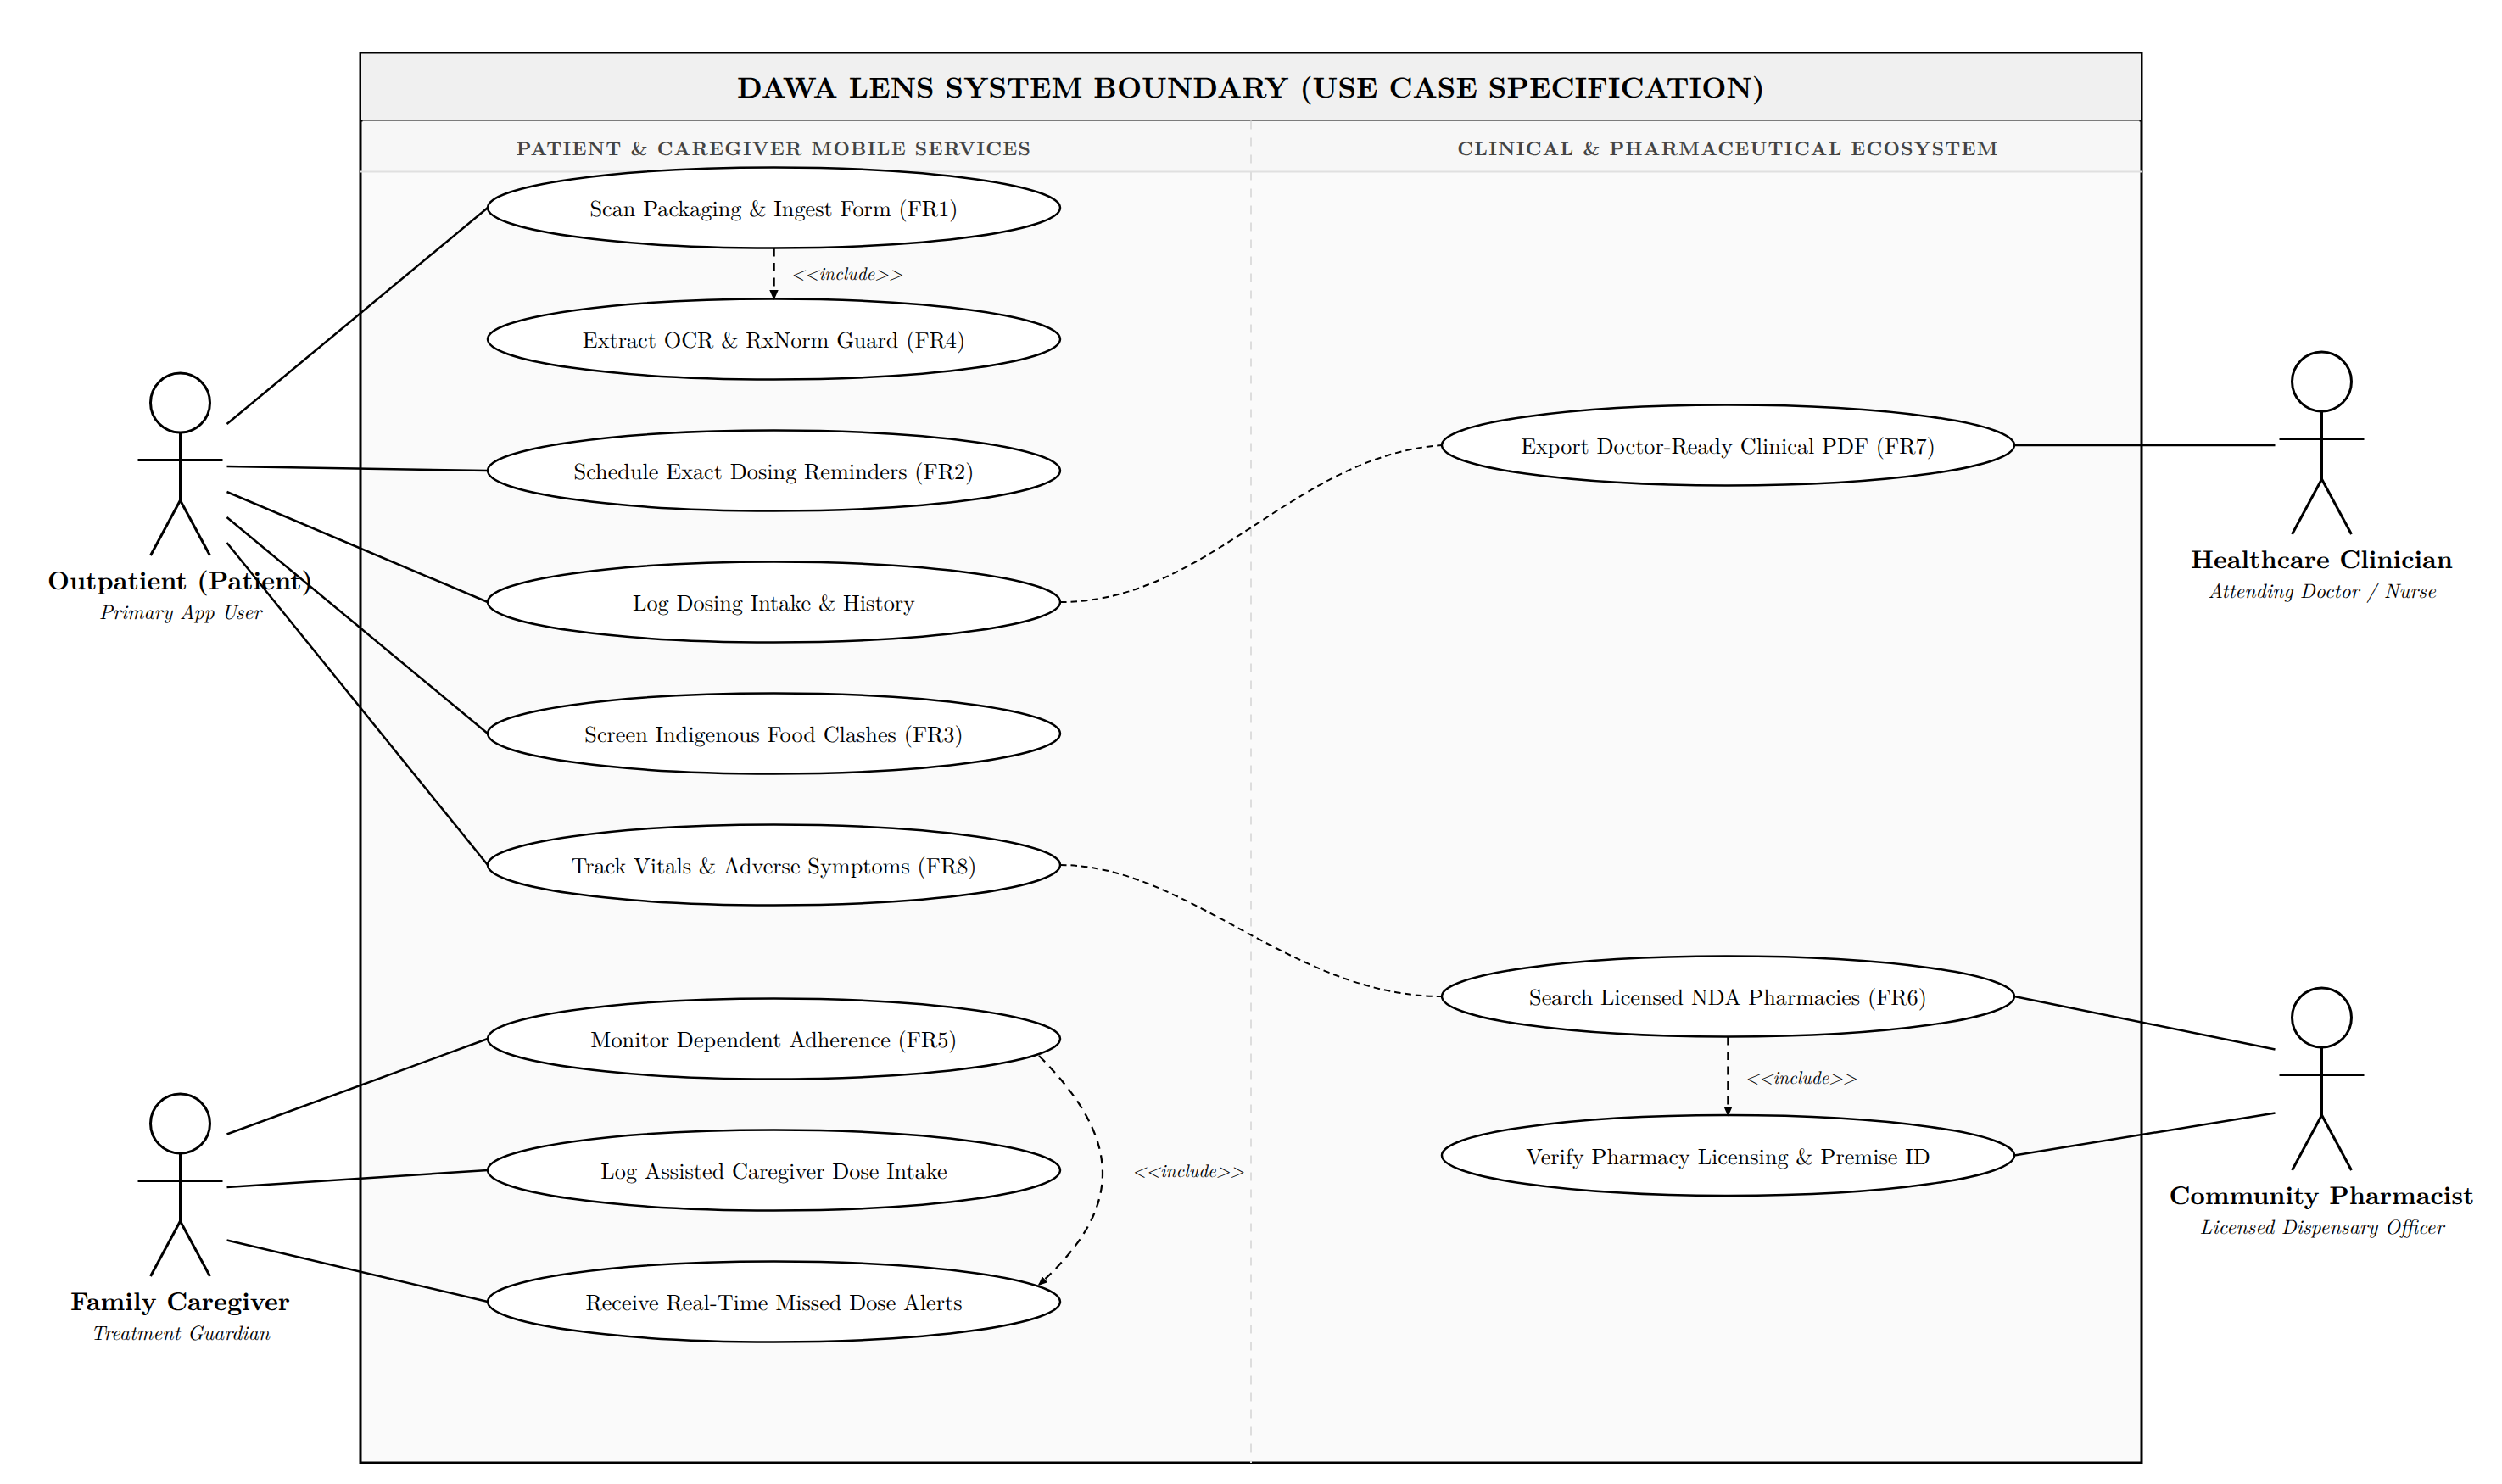
\includegraphics[width=0.95\textwidth,keepaspectratio]{figures/use_case_diagram.png}
  \caption{Multi-actor UML use case specification diagram of the Dawa Lens mobile ecosystem.}
  \label{fig:use_case}
\end{figure}

\begin{table}[!htbp]
  \centering
  \caption{Functional requirements specification and traceability matrix.}
  \label{tab:functional_requirements}
  \scriptsize
  \setlength{\tabcolsep}{3pt}
  \begin{tabularx}{\textwidth}{@{} l >{\raggedright\arraybackslash}p{2.6cm} >{\raggedright\arraybackslash}X >{\raggedright\arraybackslash}p{1.7cm} >{\centering\arraybackslash}p{1.2cm} >{\centering\arraybackslash}p{1.3cm} @{}}
    \toprule
    \textbf{Req ID} & \textbf{Requirement Title} & \textbf{The System Shall...} & \textbf{Primary Actor} & \textbf{Target Obj.} & \textbf{Priority} \\
    \midrule
    \textbf{FR1} & Automated Packaging Scanning & Capture blister packaging images and extract drug identity and dosage parameters using on-device Wasm OCR. & Patient & Obj.~(ii) & Must Have \\
    \midrule
    \textbf{FR2} & Deterministic Offline Schedule & Support interval, time-specific, and meal-aligned dosing schedules stored in local persistence. & Patient & Obj.~(iii) & Must Have \\
    \midrule
    \textbf{FR3} & Indigenous Food-Drug Screener & Screen active drugs against biochemical profiles of Ugandan staples (\textit{Matooke}, \textit{Mukene}) and issue graded warnings. & Patient & Obj.~(iii) & Must Have \\
    \midrule
    \textbf{FR4} & Drug-Drug \& Duplication Guard & Cross-reference RxNorm nomenclatures to detect adverse drug interactions and duplicate active chemicals. & Patient & Obj.~(i), (iii) & Must Have \\
    \midrule
    \textbf{FR5} & Family Caregiver Telemetry Hub & Allow primary caregivers to link dependent profiles, monitor adherence logs, and record assisted doses. & Caregiver & Obj.~(iv) & Must Have \\
    \midrule
    \textbf{FR6} & NDA Licensed Pharmacy Locator & Display geospatial maps and directories of verified community pharmacies licensed by the NDA. & Patient & Obj.~(i), (iv) & Should Have \\
    \midrule
    \textbf{FR7} & Clinical PDF Report Generator & Export longitudinal adherence percentages, missed dose records, and logged vitals as standardized PDF summaries. & Clinician & Obj.~(iv) & Should Have \\
    \midrule
    \textbf{FR8} & Health Metrics Journal & Enable logging of physiological vitals (blood pressure, blood glucose) and self-reported adverse symptoms. & Patient & Obj.~(iii) & Could Have \\
    \bottomrule
  \end{tabularx}
\end{table}

\begin{table}[!htbp]
  \centering
  \caption{Non-functional requirements specification and validation criteria.}
  \label{tab:non_functional_requirements}
  \scriptsize
  \setlength{\tabcolsep}{3pt}
  \begin{tabularx}{\textwidth}{@{} l >{\raggedright\arraybackslash}p{2.2cm} >{\raggedright\arraybackslash}X >{\raggedright\arraybackslash}p{2.4cm} >{\raggedright\arraybackslash}p{2.2cm} @{}}
    \toprule
    \textbf{Req ID} & \textbf{Quality Attribute} & \textbf{Engineering Specification / Constraint} & \textbf{Target Metric} & \textbf{Validation Method} \\
    \midrule
    \textbf{NFR1} & Offline Availability & Core scheduling, alarms, dose logging, and food screening must operate with 0\% network dependence. & 100\% offline availability & Disconnected sandbox testing \\
    \midrule
    \textbf{NFR2} & Execution Latency & Local database queries and edge OCR packaging parsing must execute without UI thread freeze. & OCR $< 2.5\,\text{s}$, DB $< 50\,\text{ms}$ & Chrome DevTools \& Android profiler \\
    \midrule
    \textbf{NFR3} & Alarm Reliability & Scheduled dose reminder alarms must fire accurately at the designated time across Doze states. & $\ge 99.5\%$ on-time trigger fidelity & Automated timing log delta analysis \\
    \midrule
    \textbf{NFR4} & System Usability & Interface must be accessible to users with low literacy, featuring high contrast and intuitive touch targets. & SUS Score $\ge 75/100$ & Standardized SUS field survey ($N=50$) \\
    \midrule
    \textbf{NFR5} & Hardware Efficiency & Background reminder scheduling and local queue processes must minimize battery drain on budget devices. & $< 3\%$ battery drain per 24 hours & Android Battery Historian benchmark \\
    \midrule
    \textbf{NFR6} & Security \& Privacy & Local health records isolated in sandboxed storage, with cloud synchronization encrypted via TLS 1.3. & Zero unencrypted plaintext transmission & Network packet inspection (Wireshark) \\
    \bottomrule
  \end{tabularx}
\end{table}

\section{Testing Strategy and Risk Analysis}

The system will undergo multi-tier verification: automated Vitest unit testing, Playwright integration testing, edge stress testing under network blackouts, and a 2-week field usability evaluation with $N=50$ participants (35 outpatients, 10 caregivers, 5 pharmacists). Table~\ref{tab:test_verification_matrix} formalizes the testing matrix, while Table~\ref{tab:risks} provides the project risk register.

\begin{table}[!htbp]
  \centering
  \caption{Multi-tier testing, verification, and validation matrix.}
  \label{tab:test_verification_matrix}
  \scriptsize
  \setlength{\tabcolsep}{3pt}
  \begin{tabularx}{\textwidth}{@{} l >{\raggedright\arraybackslash}p{2.0cm} >{\raggedright\arraybackslash}p{2.8cm} >{\raggedright\arraybackslash}X >{\centering\arraybackslash}p{1.8cm} @{}}
    \toprule
    \textbf{Test Tier} & \textbf{Subsystem Tested} & \textbf{Test Scenario / Input} & \textbf{Expected Engineering Behavior} & \textbf{Pass Metric} \\
    \midrule
    \textbf{Unit Test} & Recurrence Engine & Leap-year, timezone shift, irregular interval dosing & Deterministic computation of next dosing epoch timestamp & 100\% pass (Vitest) \\
    \midrule
    \textbf{Unit Test} & Food Interaction Guard & Co-ingestion: Enalapril + Matooke, Ciprofloxacin + Mukene & Automated trigger of Level 3 contraindication warning alert & 100\% rule recall \\
    \midrule
    \textbf{Integration} & Offline Mutation Queue & Create reminder $\to$ airplane mode $\to$ log 5 doses $\to$ reconnect & Zero data loss, with ordered FIFO flush to Firestore with retry backoff & 0\% drop rate \\
    \midrule
    \textbf{Edge Stress} & Wasm Packaging OCR & 100 degraded/curved blister foils under low ambient light ($<50\,\text{lux}$) & Binarization filter enhancement; drug name and strength parsed & CER $< 5.0\%$, latency $<2.5\,\text{s}$ \\
    \midrule
    \textbf{Edge Stress} & Local Notification Daemon & Device in Android deep Doze standby for 6 continuous hours & Exact alarm wakes CPU partial lock, and audio-visual alert fires & Trigger delta $\Delta t \le 1.0\,\text{s}$ \\
    \midrule
    \textbf{Field Pilot} & End-to-End System & 2-week continuous outpatient deployment across $N=50$ users & Longitudinal dose logging and weekly PDF report generation & SUS Score $\ge 75/100$ \\
    \bottomrule
  \end{tabularx}
\end{table}

\begin{table}[!htbp]
  \centering
  \caption{Project risk analysis and mitigation register.}
  \label{tab:risks}
  \footnotesize
  \setlength{\tabcolsep}{3.5pt}
  \begin{tabularx}{\textwidth}{@{} >{\raggedright\arraybackslash}p{2.8cm} >{\centering\arraybackslash}p{1.4cm} >{\centering\arraybackslash}p{1.3cm} >{\raggedright\arraybackslash}X @{}}
    \toprule
    \textbf{Identified Risk} & \textbf{Likelihood} & \textbf{Impact} & \textbf{Engineering Mitigation Strategy} \\
    \midrule
    \textbf{OCR Failure on Damaged Foil} & Medium & High & Implement fallback manual search with auto-suggest formulary lookup, allowing user editing of extracted OCR fields. \\
    \midrule
    \textbf{OS Background Alarm Throttling} & Medium & High & Utilize platform exact alarm permissions (\texttt{SCHEDULE\_EXACT\_ALARM}) and persistent local notification channels. \\
    \midrule
    \textbf{Intermittent Cellular Connectivity} & High & Medium & Enforce offline-first architecture with local IndexedDB persistence and transactional FIFO mutation queues. \\
    \midrule
    \textbf{Participant Attrition in Pilot} & Medium & Medium & Recruit an oversampled cohort ($N=60$) to ensure target sample size ($N=50$) is achieved, with airtime stipends provided. \\
    \midrule
    \textbf{Incomplete Local Food Data} & Low & High & Scope food rules to prominent, scientifically verified staples (\textit{Matooke}, \textit{Mukene}, \textit{G-nut sauce}) validated by clinical pharmacists. \\
    \midrule
    \textbf{Scope Creep Delaying Submission} & Medium & High & Adhere strictly to 5-sprint Agile plan, prioritizing core mobile reminder app before secondary web extensions. \\
    \bottomrule
  \end{tabularx}
\end{table}

\section{Ethical Considerations and Chapter Summary}

The study follows strict ethical procedures: written informed consent from all participants, complete anonymization of telemetry, and permanent software disclaimers stating that algorithmic alerts do not replace professional medical advice. Socially, the project advances digital inclusion, combats unregistered drug outlets via NDA registry integration, and eliminates subscription fees. Together, these methodological components establish a disciplined engineering roadmap for executing Dawa Lens at Soroti University.

\chapter{Conclusion}
\label{ch:conclusion}

This proposal has presented the engineering architecture and evaluation plan for \textbf{Dawa Lens}, an offline-first smart medicine reminder application engineered specifically to resolve the acute challenges of medication non-adherence and pharmacological safety in Uganda's outpatient healthcare environment.

The research is motivated by the pervasive public health consequences of medication mismanagement, exacerbated by unlabelled generic pharmaceutical packaging, total omission of indigenous dietary contraindications (\textit{Matooke} and \textit{Mukene}) from standard clinical databases, frequent electrical and cellular network outages, and the absence of integrated tools to verify licensed community pharmacies. Through an exhaustive review of literature and existing commercial systems, it has been established that current technologies fail in low-resource settings because they remain tethered to continuous cloud connectivity, ignore local nutritional realities, and impose unsustainable recurring subscription or hardware costs on impoverished households.

The proposed system addresses these systemic gaps through an offline-first, four-tier architecture combining on-device optical character recognition for packaging digitization, localized biochemical interaction screening, deterministic local notification scheduling, and multi-profile family caregiver synchronization. Supported by a responsive web extension for longitudinal clinical reporting, Dawa Lens transforms any standard smartphone into an intelligent, pocket-sized clinical companion that operates with zero network dependency.

The methodology formulated in Chapter~\ref{ch:methodology} provides a disciplined, structured path grounded in Design Science Research, integrating iterative Agile sprint cycles, structured unit and integration testing, and an empirical field usability evaluation across 50 participants using the standardized System Usability Scale. The proposed project is fully achievable within the allocated academic timeframe and available computing resources at Soroti University.

Upon completion, Dawa Lens is expected to deliver a measurable $\ge 35\%$ increase in scheduled dose adherence among chronic disease outpatients, eliminate preventable adverse reactions arising from indigenous dietary interactions, provide multi-generational families with shared adherence oversight, and contribute novel empirical insights to the field of mobile health engineering in Sub-Saharan Africa. The student is firmly committed to upholding the ethical responsibilities and clinical safety standards detailed in this proposal and to working under the guidance of the assigned academic supervisor, Dr. Musa Chemisto, to deliver a high-quality, production-ready final-year engineering research project.

% ---------------- References ----------------
\bibliographystyle{ieeetr}
\bibliography{references}

% ---------------- Appendices ----------------
\appendix
\chapter{Project Workplan and Implementation Schedule}
\label{app:workplan}

This appendix details the engineering workplan, activity schedule, and milestone progression required to execute Dawa Lens over the eight-month project lifecycle across the 2026/2027 academic year at Soroti University.

\section{Implementation Timeline and Milestones}

The engineering activities are structured into five sequential phases, mapped against specific deliverables in Table~\ref{tab:workplan_milestones} across the 32-week academic lifecycle.

\begin{table}[!htbp]
  \centering
  \caption{Project implementation timeline, phases, and key milestones.}
  \label{tab:workplan_milestones}
  \footnotesize
  \setlength{\tabcolsep}{3.5pt}
  \begin{tabularx}{\textwidth}{@{} >{\raggedright\arraybackslash}p{2.4cm} >{\raggedright\arraybackslash}p{2.0cm} >{\raggedright\arraybackslash}X >{\raggedright\arraybackslash}p{3.6cm} @{}}
    \toprule
    \textbf{Phase} & \textbf{Timeline} & \textbf{Major Engineering Activities} & \textbf{Key Deliverables / Milestone} \\
    \midrule
    \textbf{Phase 1: Inception} & Weeks 1--6 \newline (Oct--Nov 2026) & Literature review, stakeholder interviews, clinical guideline analysis, and requirement specification. & Approved Proposal Report and System Requirements Specification (SRS). \\
    \midrule
    \textbf{Phase 2: Architecture} & Weeks 7--12 \newline (Nov--Dec 2026) & UI/UX wireframing, IndexedDB local schema, offline queue design, and Capacitor Android runtime setup. & System Architecture Document and Prototype UI Mockups. \\
    \midrule
    \textbf{Phase 3: Development} & Weeks 13--22 \newline (Jan--Mar 2027) & Reminder scheduler, edge Tesseract.js OCR, Ugandan food-drug interaction engine, and NDA directory. & Functional Alpha Release (Android APK) and Web Clinical Extension PWA. \\
    \midrule
    \textbf{Phase 4: Evaluation} & Weeks 23--28 \newline (Mar--Apr 2027) & Unit/integration testing, offline fault benchmarking, and 2-week field usability evaluation ($N=50$) with SUS. & Quantitative Testing Report and Field Usability Evaluation Dataset. \\
    \midrule
    \textbf{Phase 5: Finalization} & Weeks 29--32 \newline (May 2027) & Empirical data analysis, final thesis drafting, supervisor review revisions, and defense preparation. & Final Research Project Report and Production Software Release. \\
    \bottomrule
  \end{tabularx}
\end{table}

\chapter{Technical Specifications and Clinical Reference Matrices}
\label{app:technical}

\section{Data Collection and Usability Instruments}
\label{app:instruments}

\subsection*{Standardized System Usability Scale (SUS)}
Participants in the field pilot ($N=50$) will complete the standardized 10-item System Usability Scale (SUS) questionnaire \cite{brooke1996sus} rated on a 5-point Likert scale (1 = Strongly Disagree to 5 = Strongly Agree): (1)~I would like to use Dawa Lens frequently for my medication, (2)~I found the application unnecessarily complex, (3)~I thought the application was easy to use, (4)~I would need the support of a technical person to use this app, (5)~The various functions were well integrated, (6)~There was too much inconsistency in the app, (7)~Most outpatients would learn to use this application very quickly, (8)~I found the application cumbersome to use, (9)~I felt confident using the application, and (10)~I needed to learn a lot of things before I could get going.

\subsection*{Semi-Structured Healthcare Worker Interview Protocol}
Community pharmacists and clinical attendants will be evaluated across five operational dimensions: (1)~frequency of patient confusion regarding generic packaging and forgotten doses, (2)~practical scanning effectiveness on generic blister strips, (3)~clinical utility of indigenous food-drug warnings (\textit{Matooke} and \textit{Mukene}), (4)~actionability of exported clinical PDF reports, and (5)~willingness to recommend Dawa Lens for chronic disease management.

\section{Local Relational Data Dictionary (IndexedDB Schema Summary)}

The client-side persistence layer is engineered using browser-standard IndexedDB managed via a custom LocalPersistence service. Table~\ref{tab:data_dictionary} summarizes the relational schema across the four core local object stores.

\begin{table}[!htbp]
  \centering
  \caption{Local client-side relational data dictionary summary (IndexedDB).}
  \label{tab:data_dictionary}
  \footnotesize
  \setlength{\tabcolsep}{3.5pt}
  \begin{tabularx}{\textwidth}{@{} >{\bfseries\raggedright\arraybackslash}p{2.4cm} >{\ttfamily\raggedright\arraybackslash}p{1.6cm} >{\raggedright\arraybackslash}p{4.4cm} >{\raggedright\arraybackslash}X @{}}
    \toprule
    \textbf{Object Store} & \textbf{PK} & \textbf{Core Fields / Attributes} & \textbf{Clinical / Engineering Purpose} \\
    \midrule
    medications & id (UUID) & name, activeIngredients, dosage, form, remainingCount, refillThreshold, verifiedNda & Local inventory of prescribed drugs, formulations, inventory counts, and NDA verification flags. \\
    \midrule
    reminders & id (UUID) & medicationId (FK), scheduledTime, daysOfWeek, mealRelation, isEnabled, notificationId & Programmed daily dosing intervals, meal alignments (before/with/after), and exact alarm notification handles. \\
    \midrule
    adherence\_logs & id (UUID) & medicationId (FK), scheduledTime, actionTime, status, loggedBy, synced & Immutable event log recording dose outcomes (taken, skipped, missed) and multi-profile caregiver attribution. \\
    \midrule
    offline\_queue & id (Auto) & operation (CRUD), collection, payload (JSON), timestamp, retryCount & Transactional FIFO mutation queue providing resilient exponential-backoff cloud synchronization. \\
    \bottomrule
  \end{tabularx}
\end{table}

\section{Reminder State Machine and Ugandan Dietary Interaction Rules}
\label{app:tables}

Medication reminders transition through four deterministic states to guarantee offline delivery: \textbf{(1)~SCHEDULED}, registered via native \texttt{SCHEDULE\_EXACT\_ALARM}, \textbf{(2)~TRIGGERED}, waking CPU partial lock and emitting an alert, \textbf{(3)~LOGGED}, recording outcome to \texttt{adherence\_logs} and updating count, and \textbf{(4)~SYNCHRONIZED}, where a background worker dequeues records to Firebase Firestore upon network reconnect. Table~\ref{tab:food_interaction_matrix} specifies the indigenous food-drug interaction rules implemented in the system.

\begin{table}[!htbp]
  \centering
  \caption{Ugandan indigenous food-drug interaction rules matrix.}
  \label{tab:food_interaction_matrix}
  \footnotesize
  \setlength{\tabcolsep}{3pt}
  \begin{tabularx}{\textwidth}{@{} >{\raggedright\arraybackslash}p{2.2cm} >{\raggedright\arraybackslash}p{2.8cm} >{\centering\arraybackslash}p{1.3cm} >{\raggedright\arraybackslash}X @{}}
    \toprule
    \textbf{Indigenous Food} & \textbf{Target Drug / Class} & \textbf{Severity} & \textbf{Biochemical Mechanism \& Automated Clinical Warning} \\
    \midrule
    \textbf{Green Bananas (\textit{Matooke})} & ACE Inhibitors (Enalapril), K$^+$-Sparing Diuretics & High (Level 3) & Dense potassium load in \textit{Matooke} (350--450mg/100g) risks hyperkalemia and cardiac dysrhythmias. \newline \textit{Warning: Avoid large portions within 2 hours of blood pressure doses.} \\
    \midrule
    \textbf{Silver Fish (\textit{Mukene})} & Fluoroquinolones (Ciprofloxacin), Tetracyclines & High (Level 3) & Calcium and iron cations form insoluble chelates, reducing antibiotic absorption by up to 70\%. \newline \textit{Warning: Do not eat Mukene 2 hours before or after antibiotic doses.} \\
    \midrule
    \textbf{Finger Millet (\textit{Kalo})} & Oral Iron Supplements (Ferrous Sulfate) & Medium (Level 2) & High phytate and tannin content binds supplemental iron, inhibiting absorption. \newline \textit{Warning: Take iron tablets with water/juice 1 hour before Kalo.} \\
    \midrule
    \textbf{Groundnut Stew (\textit{G-nut sauce})} & Antiretrovirals (Efavirenz), Lipophilic Anthelmintics & Medium (Level 2) & High fat content delays gastric emptying, altering absorption kinetics and increasing CNS side effects. \newline \textit{Warning: Take Efavirenz on an empty stomach at bedtime.} \\
    \midrule
    \textbf{Indigenous Greens (\textit{Nakati}, \textit{Dodo})} & Oral Anticoagulants (Warfarin) & High (Level 3) & Abundant Vitamin K promotes clotting factor synthesis, antagonizing Warfarin anticoagulation. \newline \textit{Warning: Maintain consistent small intake, avoiding sudden dietary surges.} \\
    \bottomrule
  \end{tabularx}
\end{table}

\end{document}
